\documentclass{beamer}

% Thème visuel
\usetheme{Madrid}
\usecolortheme{whale}

% Encodage et langue
\usepackage[utf8]{inputenc}
\usepackage[T1]{fontenc}
\usepackage[french]{babel}

% Pour afficher du code
\usepackage{listings}
\usepackage{xcolor}

% Pour afficher des images
\usepackage{graphicx}

% Style pour le code Git/bash
\lstset{
  basicstyle=\ttfamily\small,
  backgroundcolor=\color{gray!10},
  frame=single,
  breaklines=true,
  language=bash,
  keywordstyle=\color{blue},
}

% Métadonnées
\title{Simulateur de circuits analogiques en C++}
\subtitle{Projet de Première année}
\author{Enzo  \\ Aurélie  \\ Miléna }
\date{\today}

% ============================================================
\begin{document}

% Slide titre
\begin{frame}
  \titlepage
\end{frame}

% Table des matières
\begin{frame}{Sommaire}
  \tableofcontents
\end{frame}

% ============================================================
\section{Motivation}

\begin{frame}{Pourquoi ce projet existe ?}
  \begin{block}{Description}
    Ce projet permet de modéliser et de tester un circuit électronique 
    contenant des générateurs, des résistances, des diodes et des transistors 
    sans matériel physique.
  \end{block}
  \begin{block}{Notre idée}
   Nous avons simulé ce problème comme un problème d'optimisation : la minimisation
   de l'erreur quadratique sur la loi des noeuds. 
   \[ E_w(V) = \sum_{pins \in w } i_{pins} \]
   \[ E(V) =  \sum_{w \in circuit} E_w(V)^{2}\]
  \end{block}
\end{frame}

% ============================================================
\section{Architecture et choix techniques}


\begin{frame}{Structure des données}
\begin{itemize}
    \item Components (Résistance, Transistor, Diode)
    \item Wires (Fils)
    \item Const\_Wires (Fils dont la valeur de potentiel est constante)
    \item Pins (Point de connection entre un components et un wires)
    \item Circuit naïf (Contient des fils et des composants)
    \item Circuit gradient
\end{itemize}
\end{frame}

\begin{frame}[shrink=10]{Schéma d'architecture initiale}
\begin{center}
  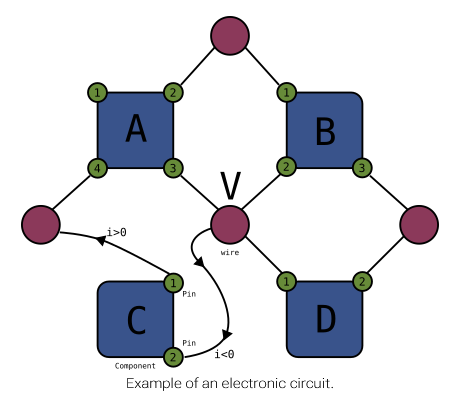
\includegraphics[width=0.8\textwidth]{pics/schema1.png}
\end{center}
\end{frame}

\begin{frame}{Schéma d'architecture finale}
\begin{columns}
  \column{0.5\textwidth}
  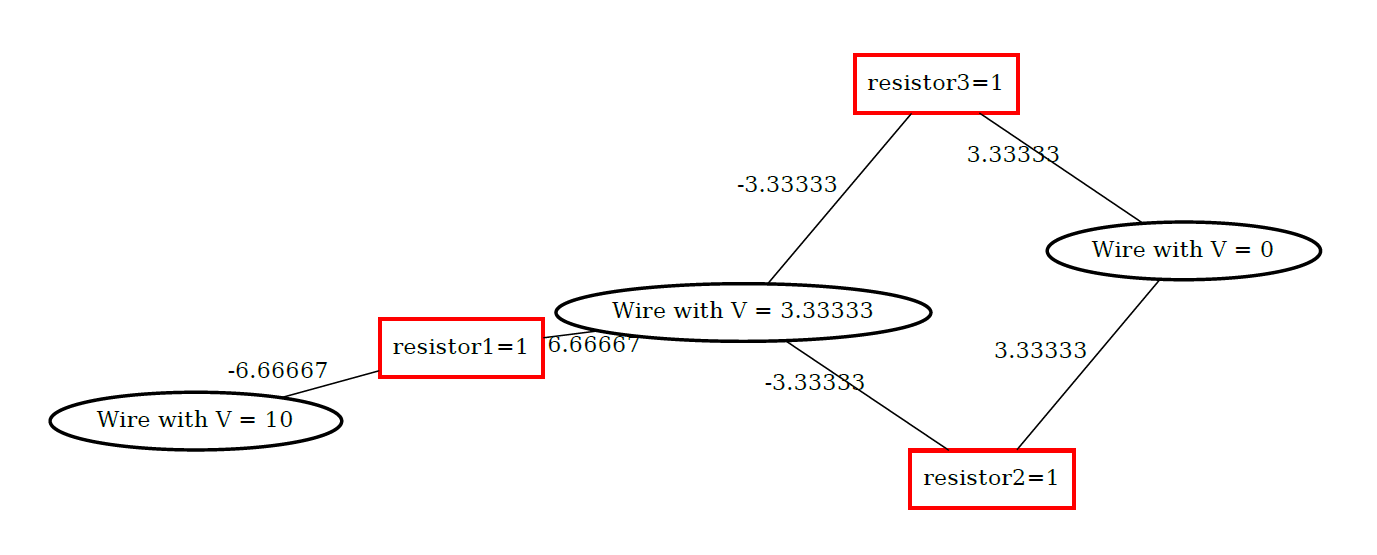
\includegraphics[width=\textwidth]{pics/schema2.png}
  \\Circuit avec des résistances en parallèle
  \column{0.5\textwidth}
  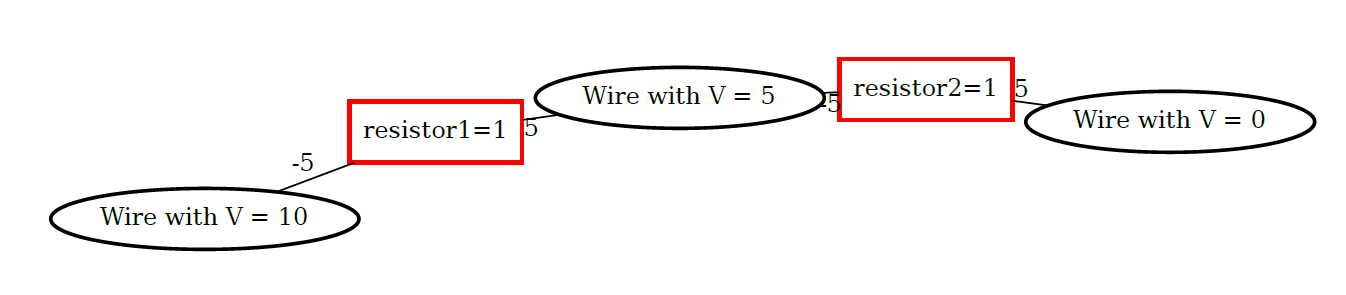
\includegraphics[width=\textwidth]{pics/schma3.png}
  \\Circuit avec des résistances en série
\end{columns}
\end{frame}

\begin{frame}[shrink = 10]{Lois physiques utilisées : Lois de Kirchhoff}
\begin{block}{Loi des noeuds ou Première loi de Kirchhoff}
  \[ \sum_{i_{entrants} \in noeud} i_{entrants} = \sum_{i_{sortants} \in noeud} i_{sortants} \]
\end{block}
\begin{block}{Interprétation}
  La loi des noeuds stipule que la somme des intensités de courant électronique
  entrant dans un noeud doit être égale à la somme des intensités de courant sortant de ce noeud.
\end{block}
\begin{block}{Loi des mailles ou Deuxième loi de Kirchhoff}
  \[ \sum_{U \in maille} U = 0\]
\end{block}
\begin{block}{Interprétation}
  La loi des mailles stipule que dans une maille (parcours fermé présent dans un circuit
  électrique), la somme des tensions est nulle.
\end{block}
\end{frame}

\begin{frame}{Lois physiques utilisées : Diode Modèle de Shockley}
  \[ I_D = I_s \left( \exp^{\frac{V_D}{n V_T}} - 1 \right) \]
  \begin{itemize}
    \item \( I_D \) courant passant dans la diode,
    \item \(I_S = 1 \cdot 10^{-12} A\) courant de saturation pris à 27\textdegree C,
    \item \( V_D \) la tension aux bornes de la diode,
    \item \( V_T = 25.852 mV\) le potentiel thermique pris à 27\textdegree C,
    \item \( n = 1\) facteur de qualité idéal.
  \end{itemize}
  
\end{frame}

\begin{frame}[shrink=10]{Lois physiques utilisées : Transistor Modèle de Ebers Moll}
  \begin{columns}
  \column{0.6\textwidth}
    \[ I_E = I_{ES} \left( \exp^{\frac{V_{BE}}{ V_T}} - 1 \right)\]
    \[ I_C = \alpha_F I_E\]
    \[ I_B = \left ( 1 - \alpha_F \right ) I_E\]
    \begin{itemize}
      \item \( I_E \) le courant émis par le transistor,
      \item \( I_C \) le courant collecteur,
      \item \( I_B \) le courant de base,
      \item \(I_{ES} = 1 \cdot 10^{-12} A\) courant de saturation pris à 27\textdegree C,
      \item \( V_{BE} \) la tension aux bornes du transistor entre le point B et le point E,
      \item \( V_T = 25.852 mV\) le potentiel thermique pris à 27\textdegree C,
      \item \( \alpha_F = 0.98\) le gain de courant .
    \end{itemize}
  \column{0.4\textwidth}
  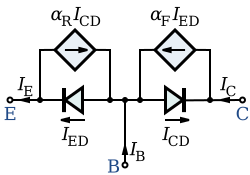
\includegraphics[width =\textwidth]{pics/schema_transistor.png}
  \end{columns}
\end{frame}

\begin{frame}[shrink=10]{Choix de conception - Naïf}
\begin{block}{Conception}
  Nous avons décidé de concevoir 2 méthodes de calcul des intensités et
  des potentiels dans le circuit.
\end{block}
\begin{block}{Principe naïf}
  Pour chaque fil libre : 
  \[ V_{libre} = V_{libre} \pm \epsilon \]
  Puis nous choisissons le \( \epsilon \) permettant de réduire au maximum l'erreur.
\end{block}
\begin{block}{Avantages}
  \begin{itemize}
    \item Simple et facile à implémenter.
    \item Utile pour déboguer un nouveau composant.
  \end{itemize}
\end{block}
\begin{block}{Inconvénients}
  \begin{itemize}
    \item Lent.
    \item Pas adapté aux circuits complexes.
  \end{itemize}
\end{block}
\end{frame}

\begin{frame}[shrink=10]{Choix de conception - Gradient}
\begin{block}{Principe gradient}
  On calcule le gradient analytique de l'erreur quadratique sur tout les fils du circuit.
  Soit :
 \[
\begin{aligned}
\nabla f(\mathbf V)
&=
\left(
\frac{\delta E}{\delta V_1},
\dots,
\frac{\delta E}{\delta V_n}
\right)
\\[0.5em]
&=
\left(
2 \sum_{w \in \mathrm{circuit}} E_w
\sum_{p \in w} \frac{\delta i_p}{\delta V_1},
\dots,
2 \sum_{w \in \mathrm{circuit}} E_w
\sum_{p \in w} \frac{\delta i_p}{\delta V_n}
\right)
\end{aligned}
\]

\end{block}
\begin{block}{Avantages}
  \begin{itemize}
    \item Rapide,
    \item Utile pour résoudre des circuits complexes.
  \end{itemize}
\end{block}
\begin{block}{Inconvénients}
  \begin{itemize}
    \item Peu précis à cause d'exponentielles qui divergent.
  \end{itemize}
\end{block}
\end{frame}

\begin{frame}{ Solution du gradient : Backtracking (pas adaptatif)}
\begin{enumerate}
\item Essayer un pas $\alpha_0$
\item Si $E(V - \alpha\nabla E) \ge E(V)$, réduire $\alpha$ (facteur $0.95$)
\item Recommencer jusqu'à trouver un pas qui diminue $E$
\item Sécurité : arrêt si $\alpha < 10^{-15}$
\end{enumerate}
\end{frame}


% ============================================================
\section{Prise en main}

\begin{frame}[fragile]{Construction d'un circuit}
\begin{lstlisting}
crt::GradCircuit c;
auto r{c += crt::make::resistor(10)};
auto d{c += crt::make::diode()};
auto [vcc, gnd] = c.make_generator(10);
auto mid = c.wire();

vcc == r->pin<0>(); 
mid == r->pin<1>();
mid == d->pin<0>(); 
gnd == d->pin<1>();
solve<Grad_Desc>(c);
\end{lstlisting}
\end{frame}

\begin{frame}[fragile]{Présentation des résultats}
Nous avons également une partie \textbf{utilities}
\begin{lstlisting}
  solve<Grad_Desc>(circuit);
    {
        
        std::ofstream file_bfsolve("circuit_ex8_grad-solved.dot");
        file_bfsolve << circuit;
        crt::utilities::show("circuit_ex8_grad-solved.dot");
    }
\end{lstlisting}
\end{frame}

\section{Concepts C++20}
\begin{frame}[fragile]{Concepts}
\begin{lstlisting}
template <typename Circuit>
concept Grad_Desc = NaiveSolve_Circuit<Circuit> &&
    requires(Circuit c) {
        { c.compute_grad() } -> std::ranges::range;
    };
\end{lstlisting}
\begin{itemize}
\item Erreurs de typage détectées à la compilation
\item Messages clairs
\item Oriente l'utilisateur vers la bonne classe de circuit
\end{itemize}
\end{frame}


% ============================================================
\section{Résultats et validation}

\begin{frame}[shrink = 10]{Exemple 1}
  \begin{center}
  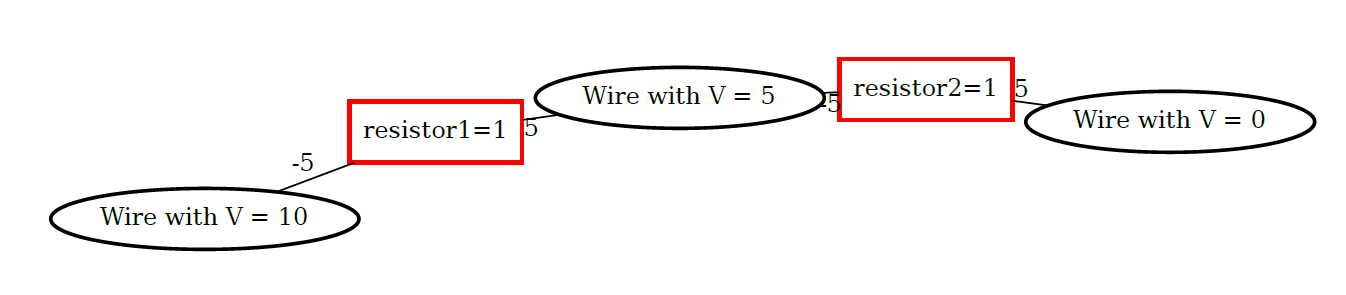
\includegraphics[width=\textwidth]{pics/schma3.png}
  \\Circuit avec 1 générateur 10 V, 2 résistance à 1$\Omega$ en série
  \end{center}
\end{frame}

\begin{frame}{Résolution}
\begin{columns}[T]
  \column{0.5\textwidth}
  \textbf{Résolution Naïve}
    \begin{itemize}
    \item Erreur finale \( 4.7606 \cdot 10^{-19}\)
    \item Convergence en \(5\space000\space000\) itérations
    \end{itemize}
  \column{0.5\textwidth}
  \textbf{Résolution avec le gradient}
    \begin{itemize}
    \item Erreur finale \( 2.8519 \cdot 10^{-14}\)
    \item Convergence en \(139\) itérations
    \end{itemize}
  \end{columns}
\end{frame}


\begin{frame}[shrink = 10]{Evolution}
  \begin{center}
  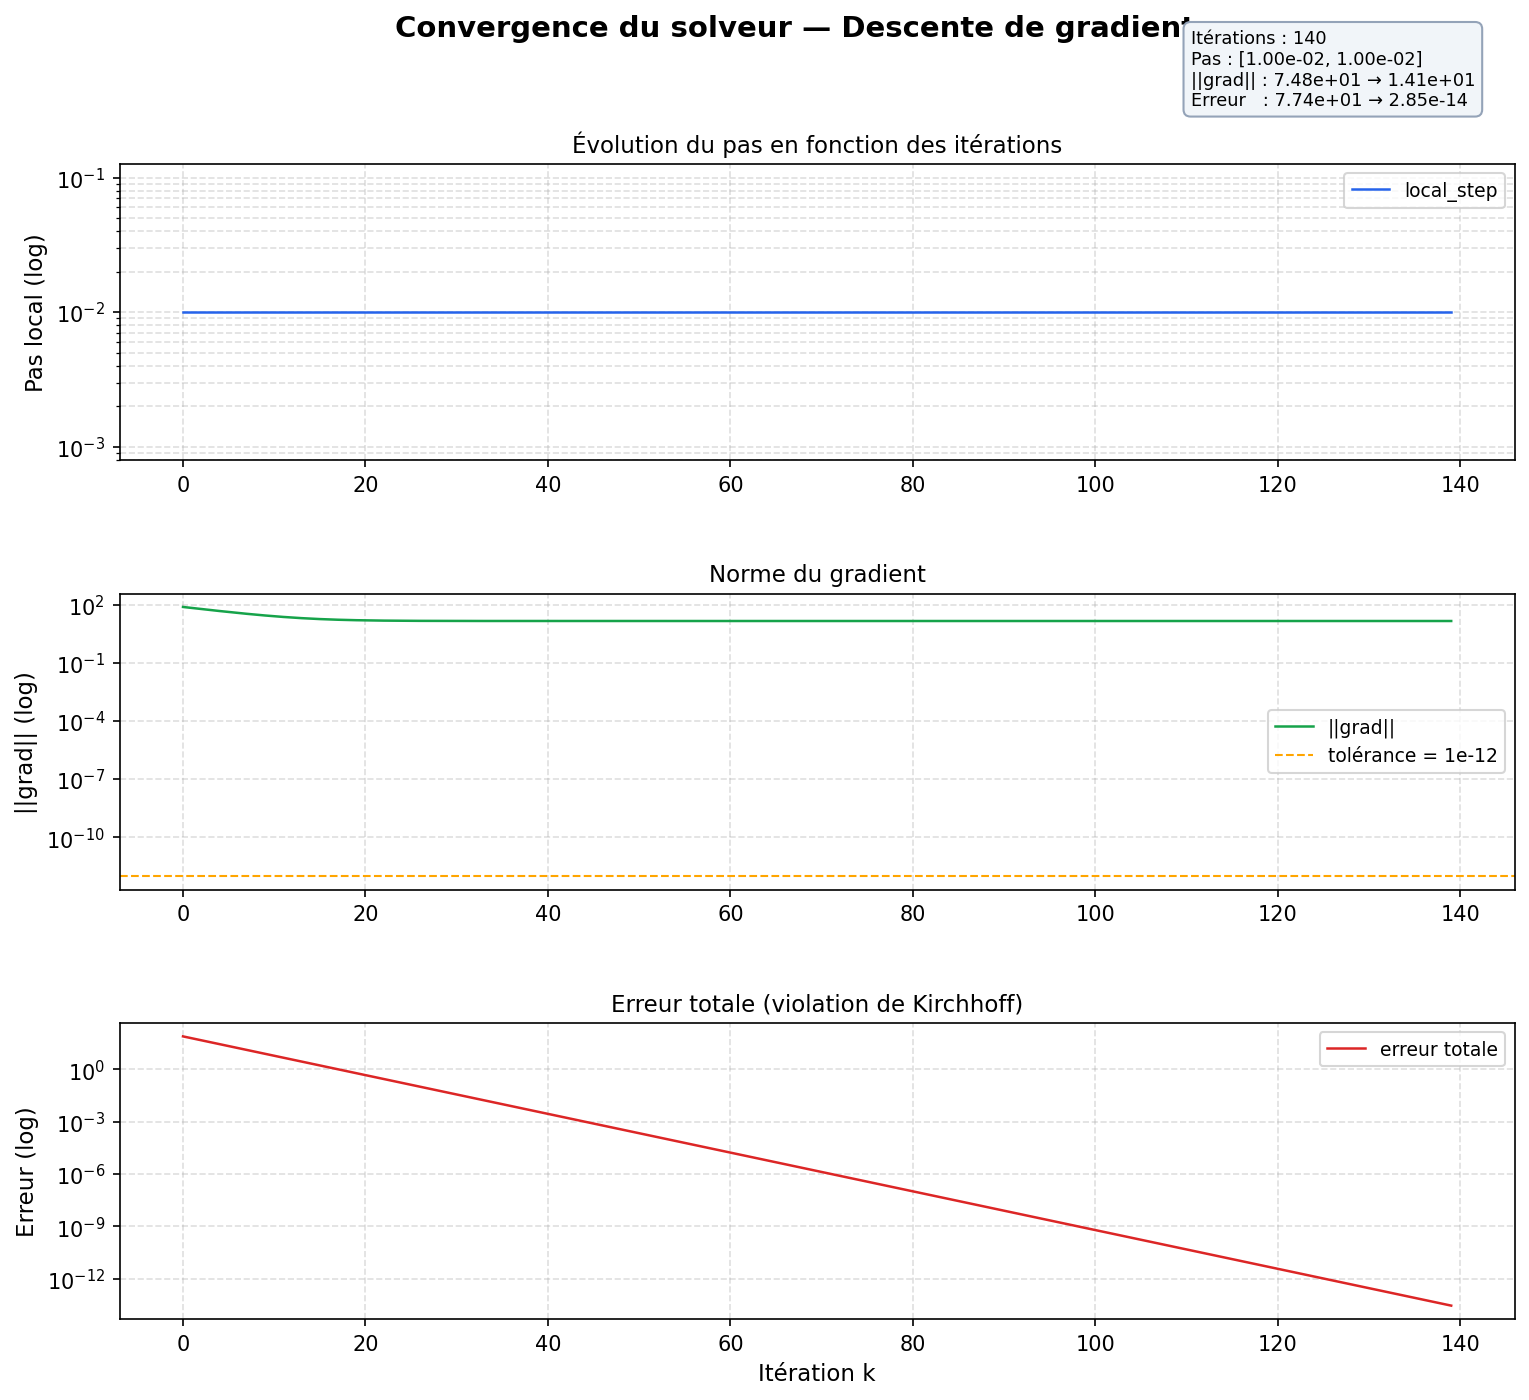
\includegraphics[width=\textwidth]{pics/evol_grad1.png}
  \end{center}
\end{frame}


\begin{frame}{Exemple 2 - Résolution}
  Circuit avec 1 générateur 5 V, 1 résistance à 1$\Omega$ et 1 diode en série. \\

\begin{columns}[T]
  \column{0.5\textwidth}
  \textbf{Résolution Naïve}
    \begin{itemize}
    \item Erreur finale \( 0.0018 \)
    \item Convergence en \(201\space512\) itérations
    \item Problème à cause de la divergence de l'exponentielle de l'intensité travarsant la diode.
    \end{itemize}
  \column{0.5\textwidth}
  \textbf{Résolution avec le gradient}
    \begin{itemize}
    \item Erreur finale \( 0.0021\)
    \item Convergence en \(106\) itérations
    \end{itemize}
  \end{columns}
\end{frame}

\begin{frame}[shrink = 10]{Schema}
  \begin{columns}
    \column{0.5\textwidth}
    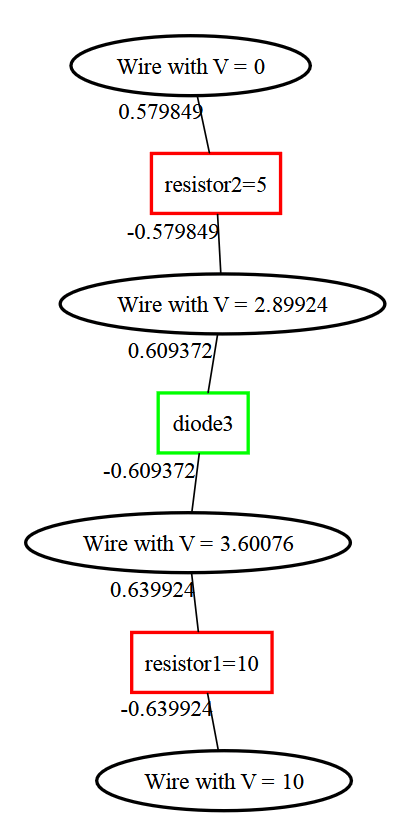
\includegraphics[width=0.8\textwidth]{pics/schema4_naive2.png}
    \\ Circuit lors de la résolution naive
    \column{0.5\textwidth}
    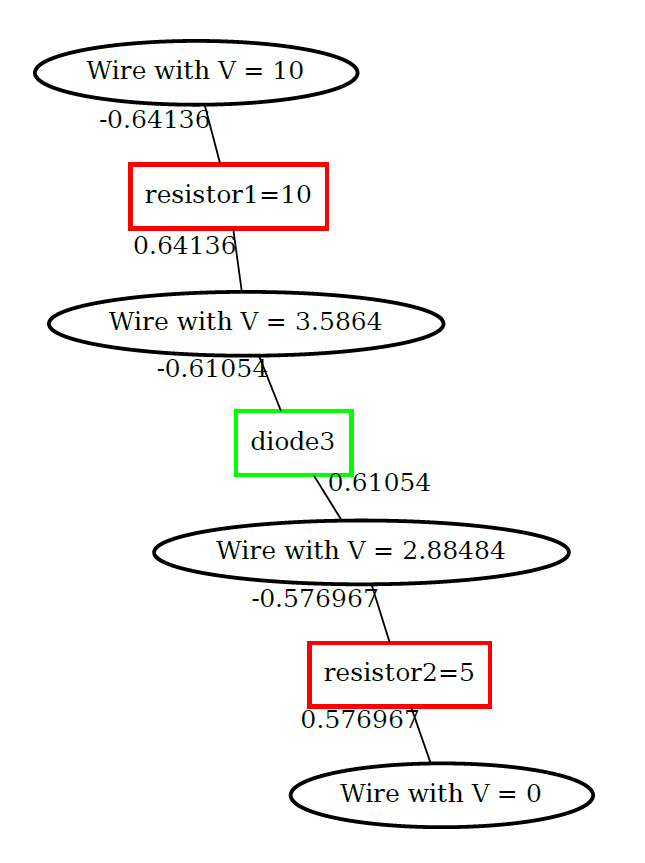
\includegraphics[width=\textwidth]{pics/schema4_grad.png}
    \\ Circuit lors de la résolution avec le gradient
  \end{columns}
\end{frame}

\begin{frame}[shrink = 10]{Evolution}
  \begin{center}
  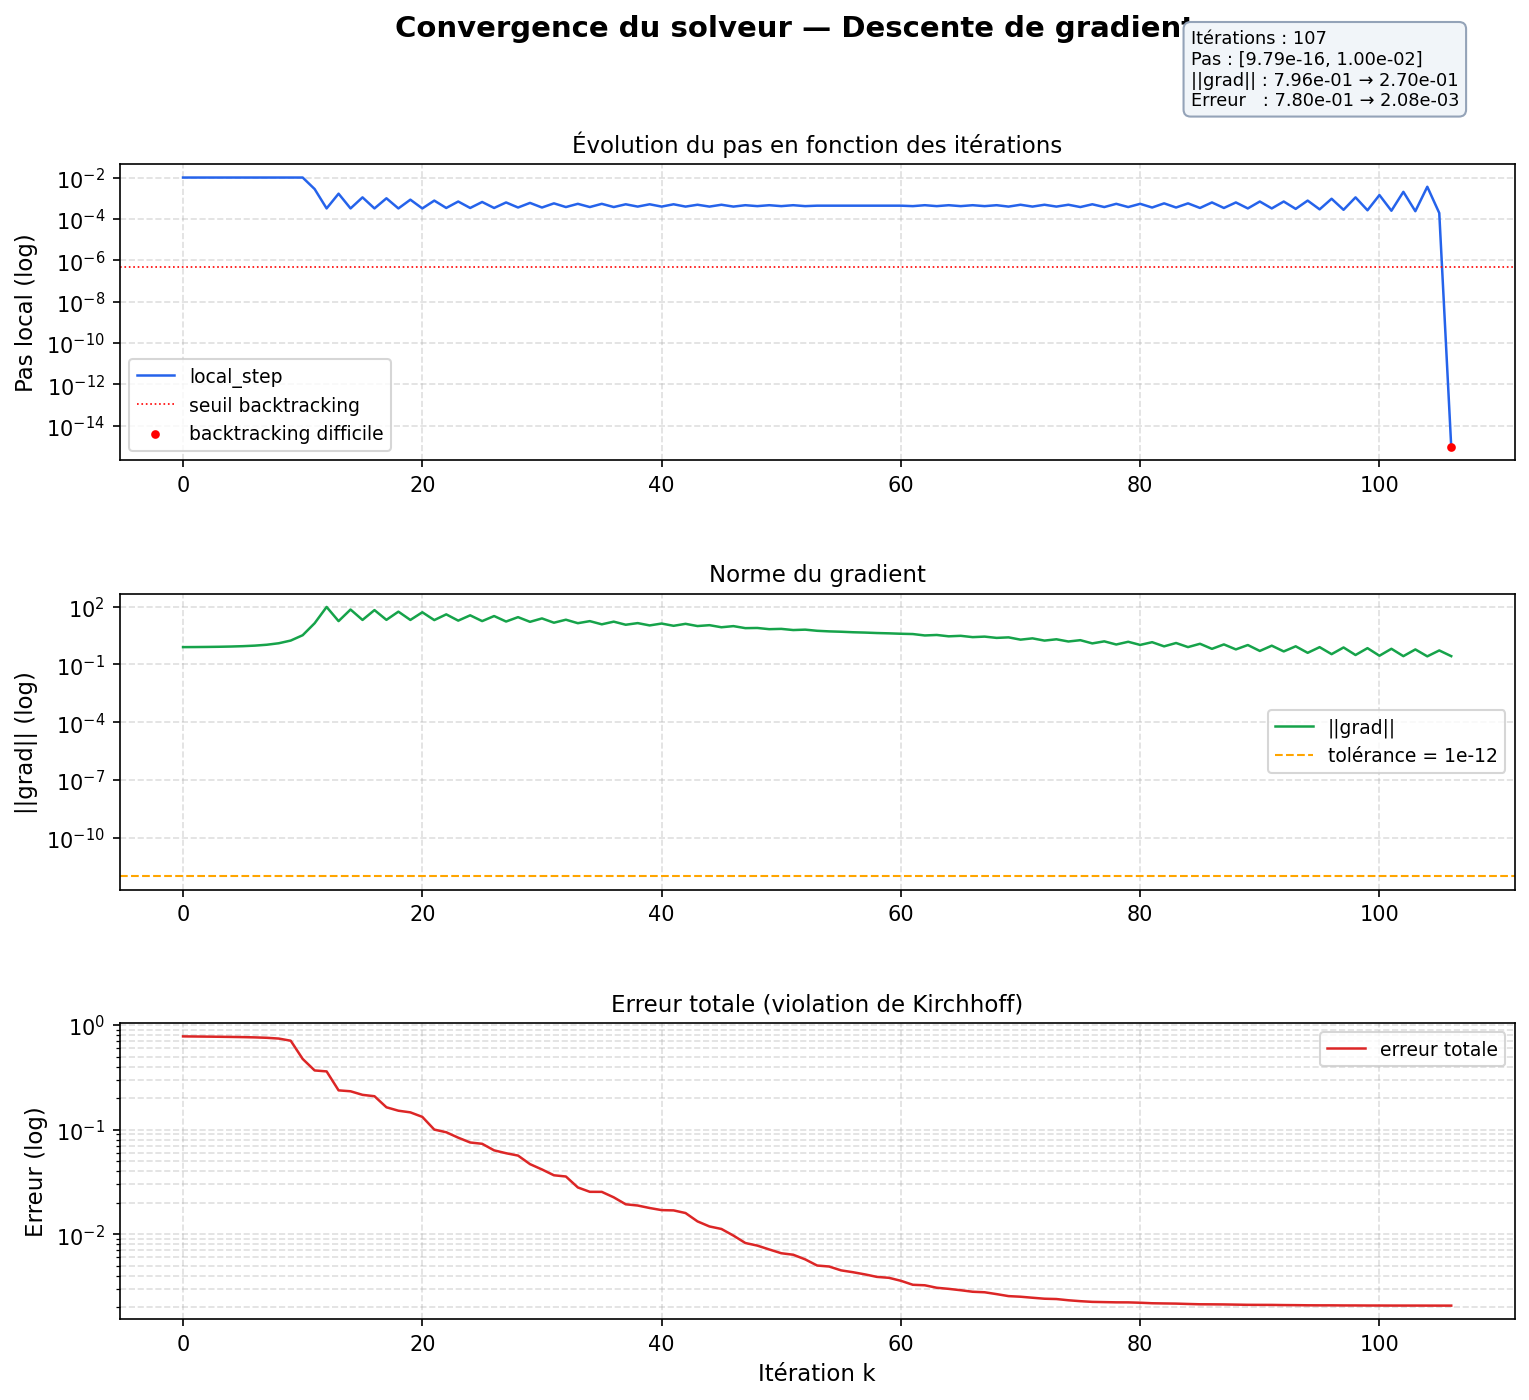
\includegraphics[width=\textwidth]{pics/evol_grad2.png}
  \end{center}
\end{frame}


\begin{frame}{Exemple 3 - Résolution}
  Circuit avec 1 générateur 5 V, 3 résistance à 2$\Omega$ et 1 transistor. \\
  
\begin{columns}[T]
  \column{0.5\textwidth}
  \textbf{Résolution Naïve}
    \begin{itemize}
    \item Erreur finale \( 1.0418 \)
    \item Convergence en \(24\space 315\space 600\) itérations
    \item Problème à cause de la divergence de l'exponentielle de l'intensité traversant le transistor.
    \end{itemize}
  \column{0.5\textwidth}
  \textbf{Résolution avec le gradient}
    \begin{itemize}
    \item Erreur finale \( 9.35585\)
    \item Convergence en \(5\space258\) itérations
    \end{itemize}
  \end{columns}
\end{frame}

\begin{frame}[shrink = 10]{Schema}
  \begin{columns}
    \column{0.5\textwidth}
    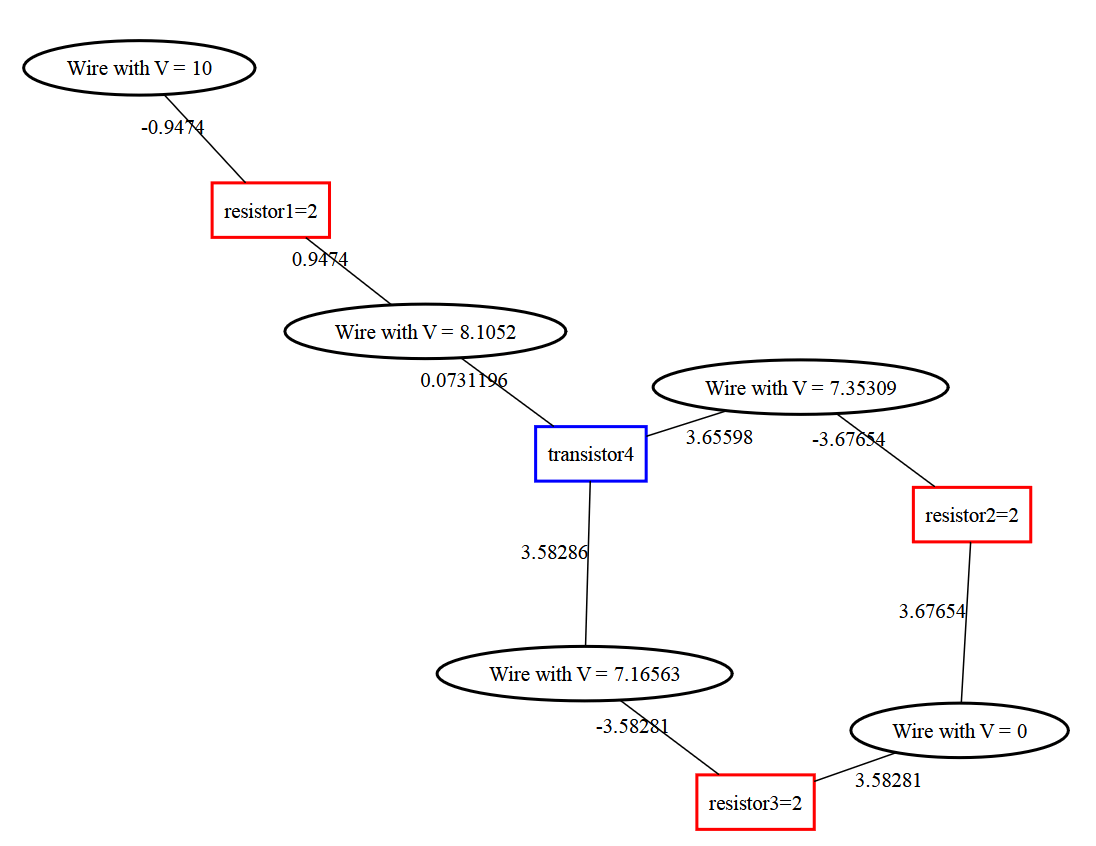
\includegraphics[width=\textwidth]{pics/schema5_naive2.png}
    \\ Circuit lors de la résolution naive
    \column{0.5\textwidth}
    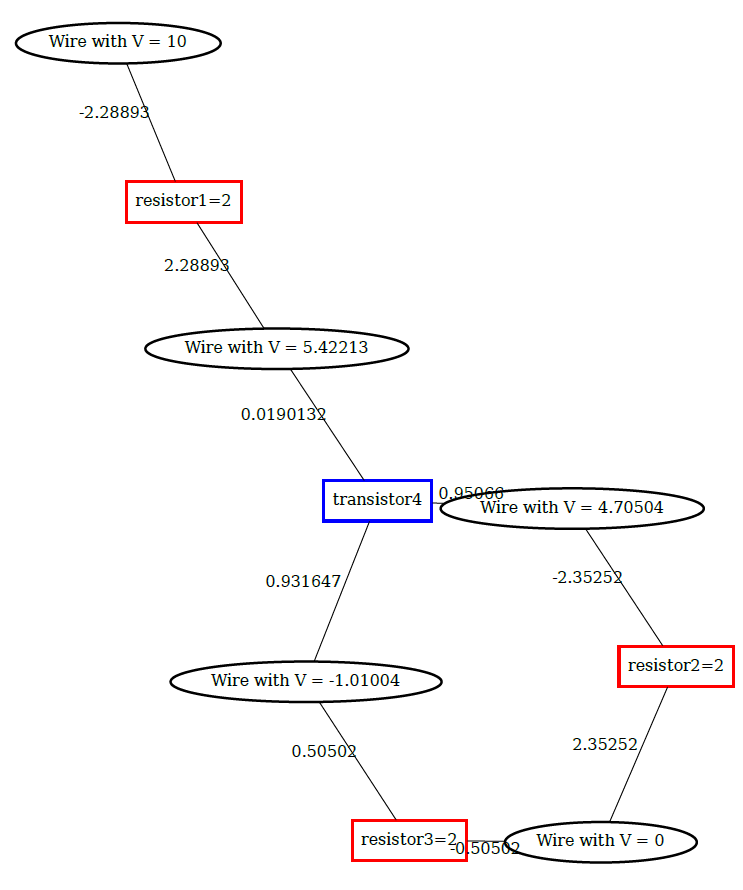
\includegraphics[width=\textwidth]{pics/shema5_grad.png}
    \\ Circuit lors de la résolution avec le gradient
  \end{columns}
\end{frame}

\begin{frame}[shrink = 10]{Evolution}
  \begin{center}
  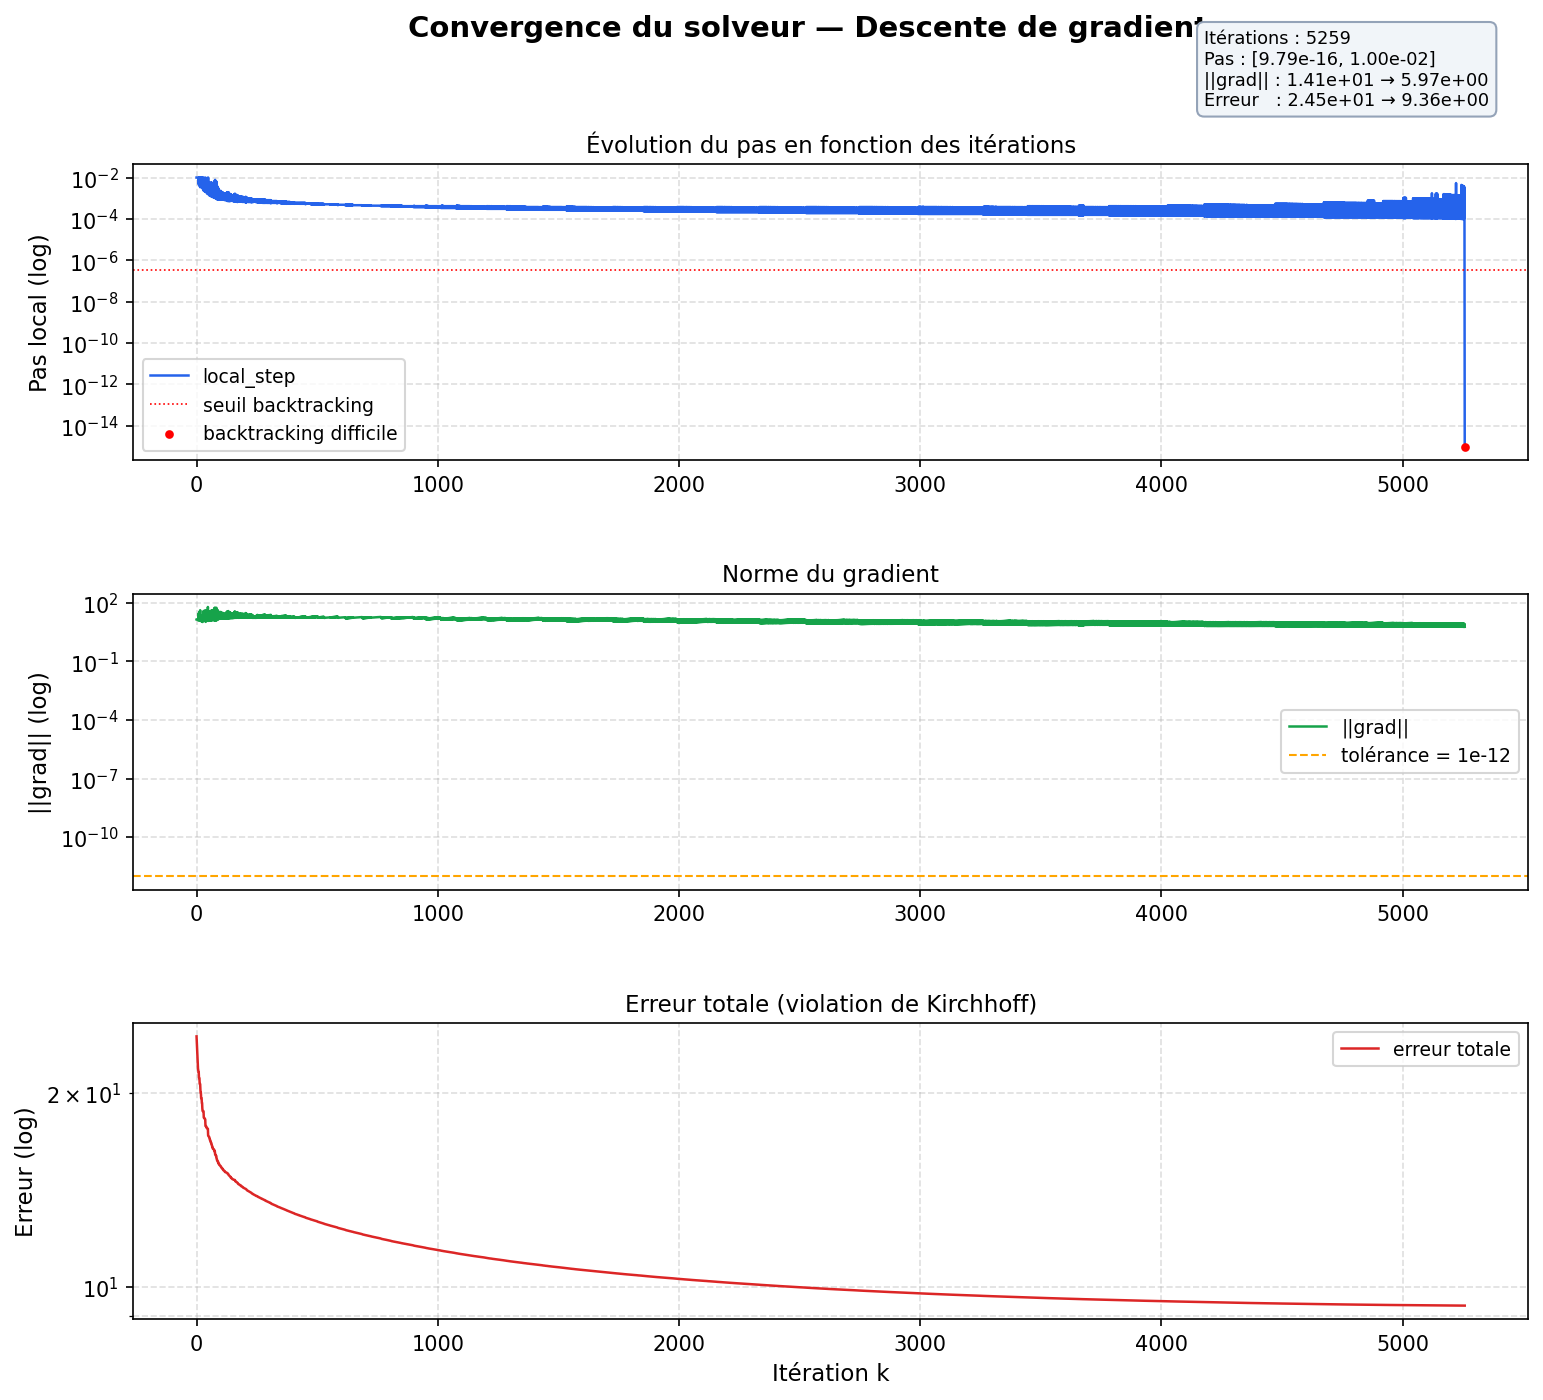
\includegraphics[width=\textwidth]{pics/evol_grad3.png}
  \end{center}
\end{frame}



\begin{frame}{Validation}
    \begin{block}{Réel circuit physique}
      Nous sommes encore loin du temps de calcul d'un circuit physique \( \approx 1 \mu s\).
    \end{block}
    \begin{block}{Succès}
      Cependant, nous avons quand même réussi à modéliser les diodes, les résistances et les transistor assez proches de leur modèle réel.
      La surchage des opérateurs \textbf{==} et \textbf{+=} est esthétique lors de la conception des circuits.
    \end{block}
    \begin{block}{Limites}
      Nos programmes ne gèrent pas les minimums locaux. 
    \end{block}

\end{frame}



\section{Pistes d'amélioration}
\begin{frame}{Ce que l'on peut ajouter}
\begin{itemize}
\item \textbf{Newton‑Raphson} : Jacobien disponible via \texttt{d()}, convergence quadratique
\item \textbf{Régime transitoire} : condensateurs, bobines
\item \textbf{Interface graphique} (saisie schématique)
\end{itemize}
\end{frame}

% ============================================================
\section{Conclusion}
\begin{frame}{Conclusion}
\begin{itemize}
\item Bibliothèque de simulation analogique en C++20
\item Architecture modulaire et extensible
\item Deux solveurs : naïf et gradient avec backtracking
\item Infrastructure prête pour Newton‑Raphson
\end{itemize}
Merci de votre attention. Des questions ?
\end{frame}
\end{document}
